\chapter{Errors}
\subsection{Pdf Viewer Compilation Error in TeXnicCenter}
Auf die Karte Build → Define Output Profiles klicken. Im neuen Fenster auf Latex→PDF klicken und dann auf die Karte Viewer. Statt \textit{acroview} wie Server zu haben, muss man \textit{acroviewAnn} schreiben. Dabei ist \textit{nn} ein Versionsjahr von Acrobat. Z.B. 2024 → nn=24 Konfiguration von PDF Viewer in TeXnicCenter ist nötig.  

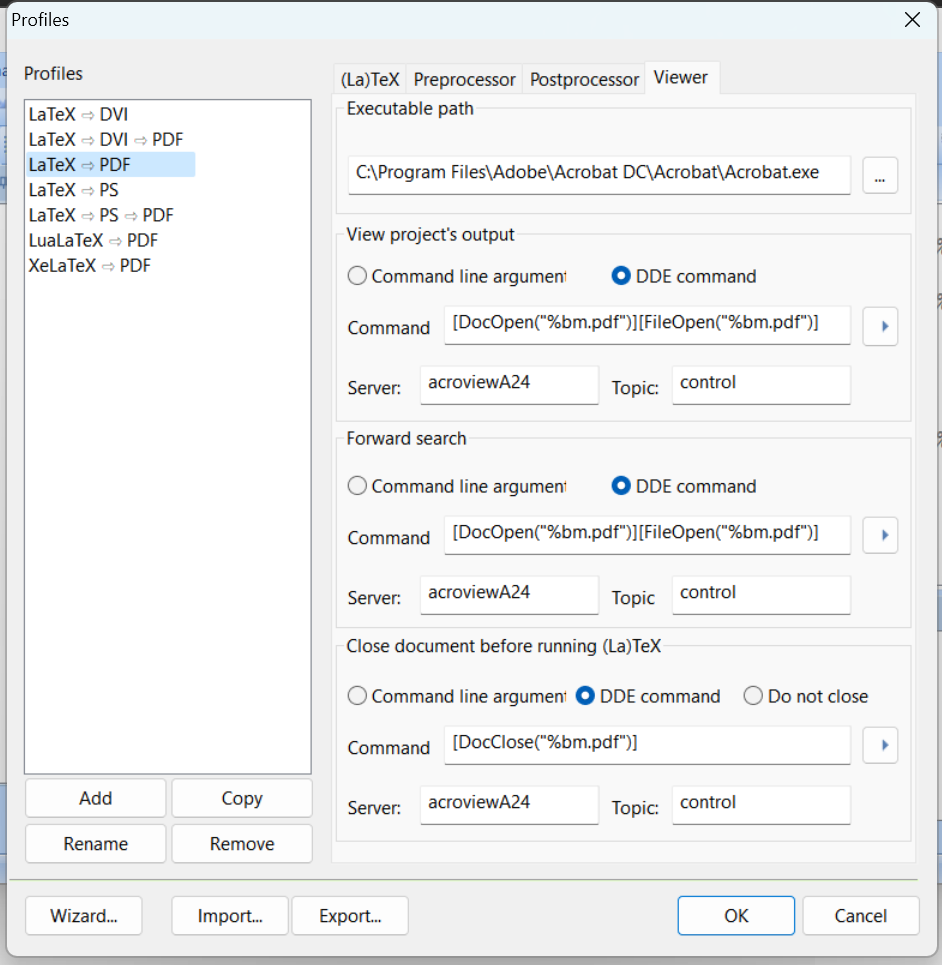
\includegraphics[width=\linewidth]{LTX_Sources/texniccenter-pdf-config.png}